% Options for packages loaded elsewhere
\PassOptionsToPackage{unicode}{hyperref}
\PassOptionsToPackage{hyphens}{url}
\PassOptionsToPackage{dvipsnames,svgnames*,x11names*}{xcolor}
%
\documentclass[
  12pt,
  ,
  a4paper]{article}
\usepackage{lmodern}
\usepackage{amssymb,amsmath}
\usepackage{ifxetex,ifluatex}
\ifnum 0\ifxetex 1\fi\ifluatex 1\fi=0 % if pdftex
  \usepackage[T1]{fontenc}
  \usepackage[utf8]{inputenc}
  \usepackage{textcomp} % provide euro and other symbols
\else % if luatex or xetex
  \usepackage{unicode-math}
  \defaultfontfeatures{Scale=MatchLowercase}
  \defaultfontfeatures[\rmfamily]{Ligatures=TeX,Scale=1}
\fi
% Use upquote if available, for straight quotes in verbatim environments
\IfFileExists{upquote.sty}{\usepackage{upquote}}{}
\IfFileExists{microtype.sty}{% use microtype if available
  \usepackage[]{microtype}
  \UseMicrotypeSet[protrusion]{basicmath} % disable protrusion for tt fonts
}{}
\makeatletter
\@ifundefined{KOMAClassName}{% if non-KOMA class
  \IfFileExists{parskip.sty}{%
    \usepackage{parskip}
  }{% else
    \setlength{\parindent}{0pt}
    \setlength{\parskip}{6pt plus 2pt minus 1pt}}
}{% if KOMA class
  \KOMAoptions{parskip=half}}
\makeatother
\usepackage{xcolor}
\IfFileExists{xurl.sty}{\usepackage{xurl}}{} % add URL line breaks if available
\IfFileExists{bookmark.sty}{\usepackage{bookmark}}{\usepackage{hyperref}}
\hypersetup{
  pdftitle={Rapport},
  pdfauthor={Alain Quartier-la-Tente},
  pdflang={english},
  colorlinks=true,
  linkcolor=Maroon,
  filecolor=Maroon,
  citecolor=Blue,
  urlcolor=blue,
  pdfcreator={LaTeX via pandoc}}
\urlstyle{same} % disable monospaced font for URLs
\usepackage[margin=1in]{geometry}
\usepackage{longtable,booktabs}
% Correct order of tables after \paragraph or \subparagraph
\usepackage{etoolbox}
\makeatletter
\patchcmd\longtable{\par}{\if@noskipsec\mbox{}\fi\par}{}{}
\makeatother
% Allow footnotes in longtable head/foot
\IfFileExists{footnotehyper.sty}{\usepackage{footnotehyper}}{\usepackage{footnote}}
\makesavenoteenv{longtable}
\usepackage{graphicx,grffile}
\makeatletter
\def\maxwidth{\ifdim\Gin@nat@width>\linewidth\linewidth\else\Gin@nat@width\fi}
\def\maxheight{\ifdim\Gin@nat@height>\textheight\textheight\else\Gin@nat@height\fi}
\makeatother
% Scale images if necessary, so that they will not overflow the page
% margins by default, and it is still possible to overwrite the defaults
% using explicit options in \includegraphics[width, height, ...]{}
\setkeys{Gin}{width=\maxwidth,height=\maxheight,keepaspectratio}
% Set default figure placement to htbp
\makeatletter
\def\fps@figure{htbp}
\makeatother
\setlength{\emergencystretch}{3em} % prevent overfull lines
\providecommand{\tightlist}{%
  \setlength{\itemsep}{0pt}\setlength{\parskip}{0pt}}
\setcounter{secnumdepth}{5}
%début contraintes ensae
\usepackage{pdfpages, setspace, mathptmx} %times roman
\onehalfspacing 
\makeatletter
\def\@maketitle{%
  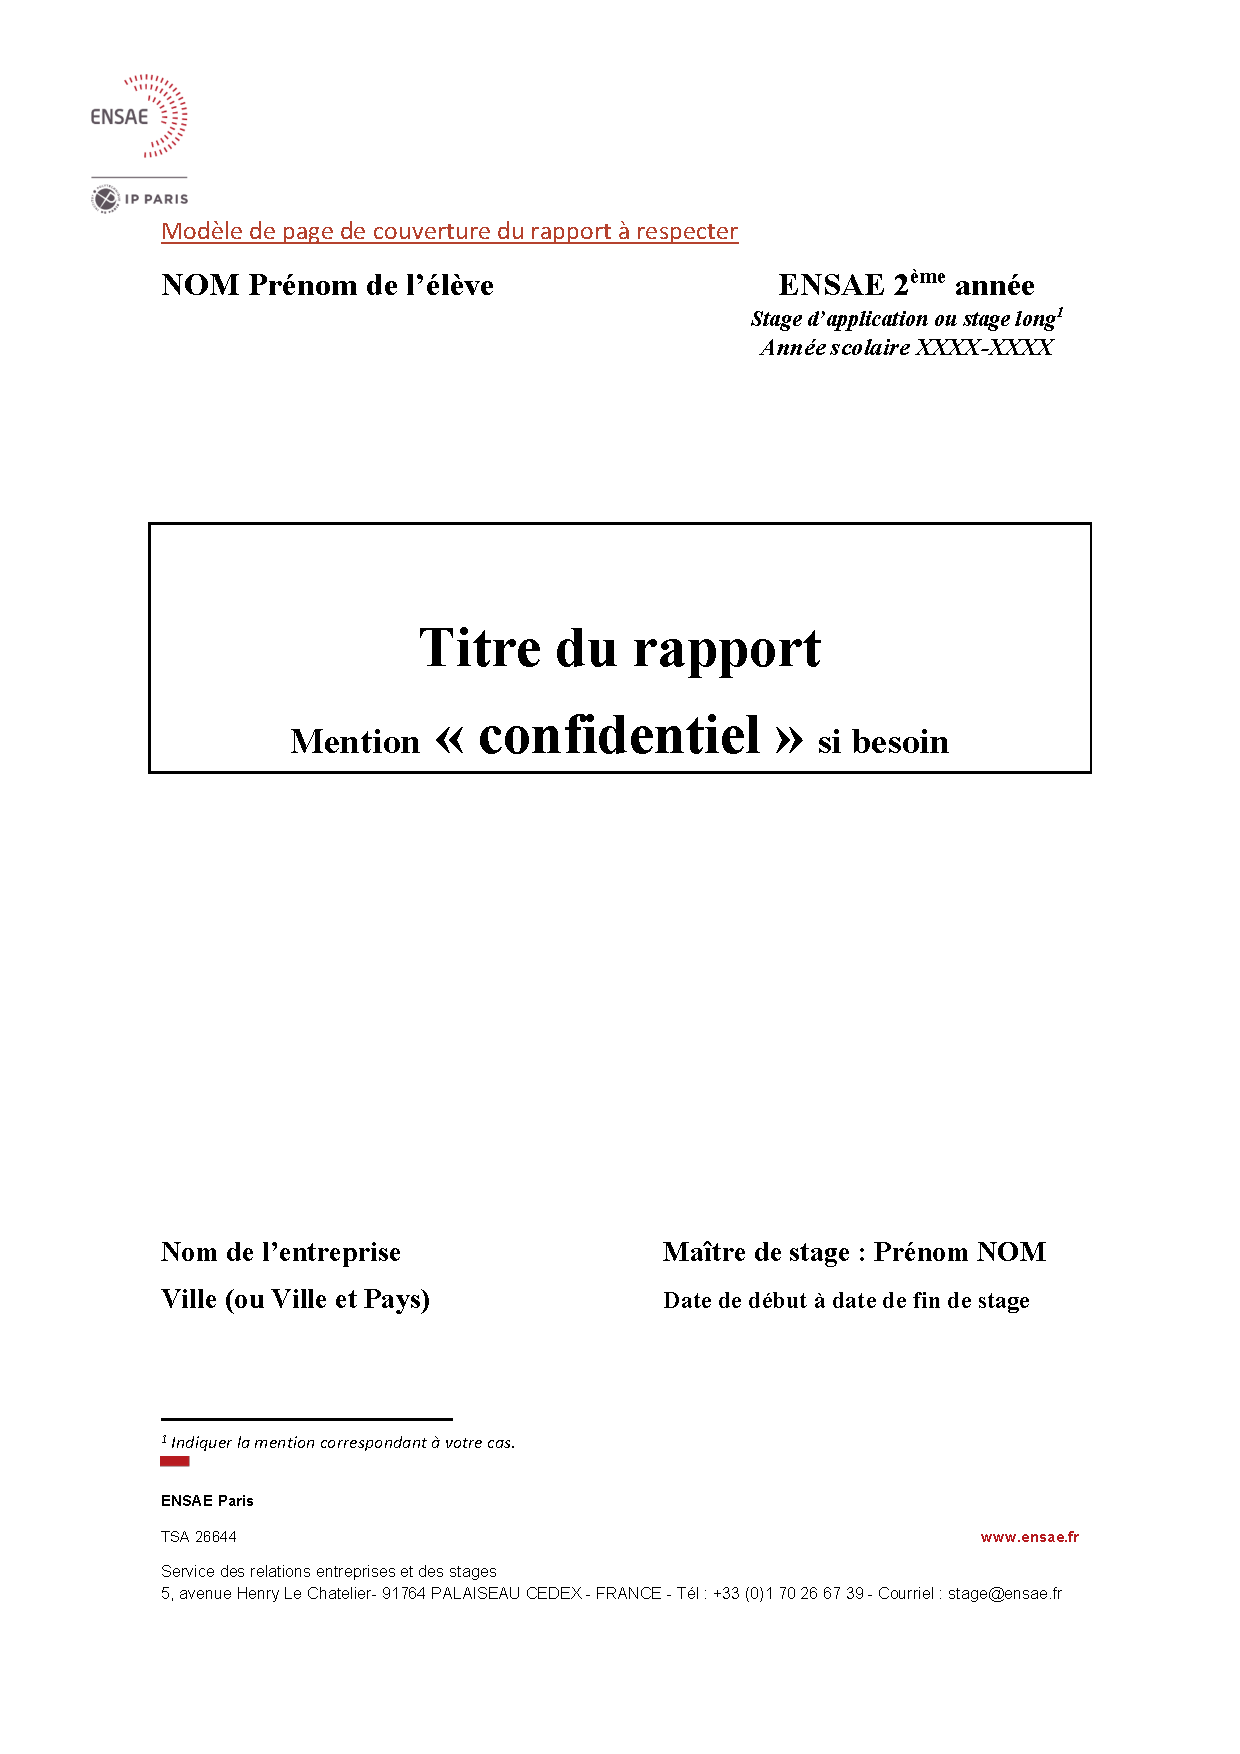
\includepdf[fitpaper=true, pages=-]{img/pdg.pdf}
}
\makeatother% cinsérer page de garde

\usepackage{stmaryrd}
\usepackage{multicol}
\usepackage{graphicx}
\usepackage{animate, dsfont, here, xspace}

%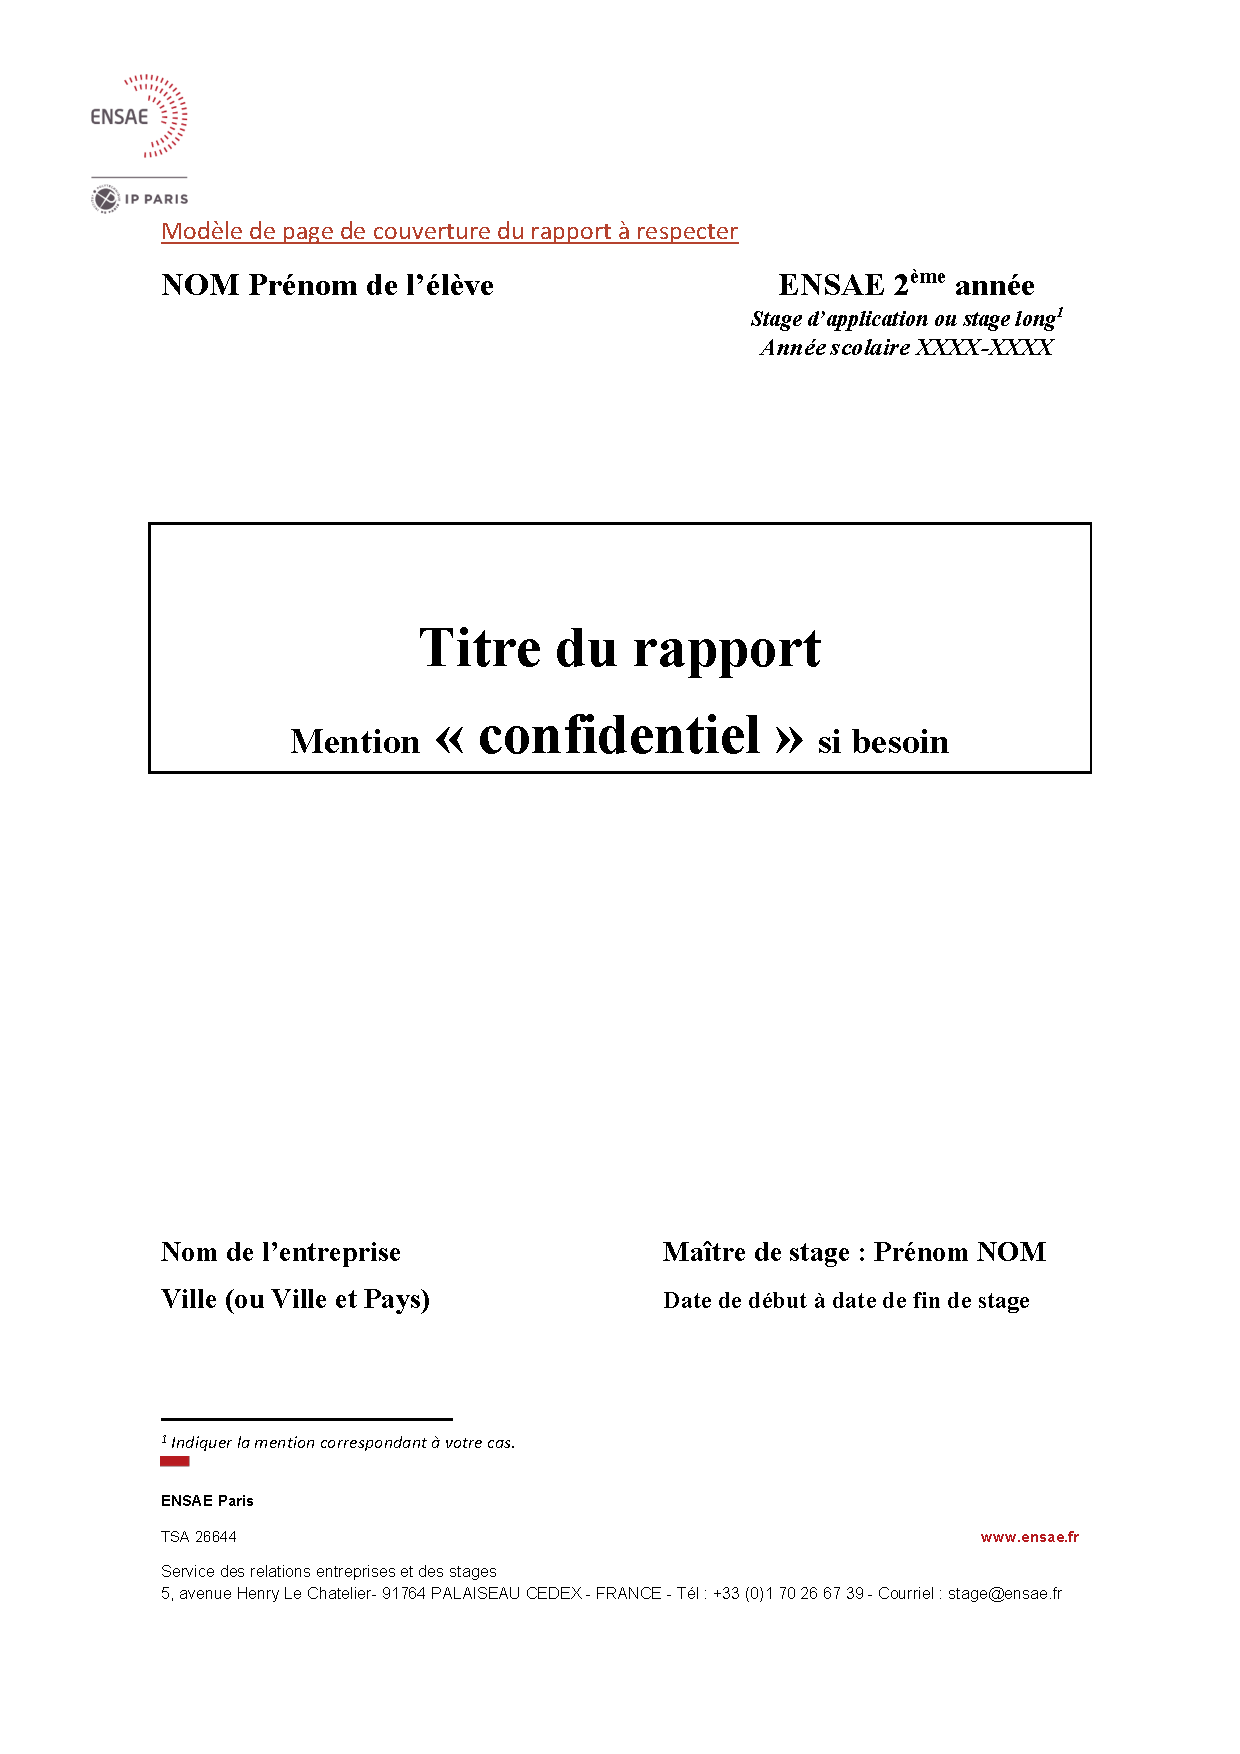
\includepdf[fitpaper=true, pages=-]{img/pdg.pdf}


\DeclareMathOperator{\e}{e}
\renewcommand{\P}{\mathds{P}} %Apparement \P existe déjà ?
\newcommand\N{\mathds{N}}
\newcommand\R{\mathds{R}}
%\newcommand\C{\mathds{C}}
%\newcommand\Z{\mathds{Z}}


\newcommand\1{\mathds{1}}
\newcommand{\E}[2][]{{\mathds{E}}_{#1}
  \def\temp{#2}\ifx\temp\empty
  \else
  \left[#2\right]
  \fi
}
\newcommand{\V}[2][]{{\mathds{V}}_{#1}
  \def\temp{#2}\ifx\temp\empty
  \else
  \left[#2\right]
  \fi
}
\newcommand\ud{\,\mathrm{d}}
\usepackage{booktabs}
\usepackage{longtable}
\usepackage{array}
\usepackage{multirow}
\usepackage{wrapfig}
\usepackage{float}
\usepackage{colortbl}
\usepackage{pdflscape}
\usepackage{tabu}
\usepackage{threeparttable}
\usepackage{threeparttablex}
\usepackage[normalem]{ulem}
\usepackage{makecell}
\usepackage{xcolor}
\ifxetex
  % Load polyglossia as late as possible: uses bidi with RTL langages (e.g. Hebrew, Arabic)
  \usepackage{polyglossia}
  \setmainlanguage[]{}
\else
  \usepackage[shorthands=off,main=]{babel}
\fi

\title{Rapport}
\author{Alain Quartier-la-Tente}
\date{6/17/2020}

\begin{document}
\maketitle

{
\hypersetup{linkcolor=}
\setcounter{tocdepth}{3}
\tableofcontents
}
\newpage

\hypertarget{introduction}{%
\section{Introduction}\label{introduction}}

\hypertarget{moving-average-and-filters}{%
\section{Moving average and filters}\label{moving-average-and-filters}}

A lot of papers describes the definition and the properties of moving average and linear filters (see for example (Ladiray 2018)).
He we summarize some of the main results.

Let \(p\) et \(f\) two integers, a moving average \(M_\theta\) or \(M\) is defined by a set of coefficients \(\theta=(\theta_{-p},\dots,\theta_{f})'\) such as:
\[
M(X_t)=\sum_{k=-p}^{+f}\theta_kX_{t+k}
\]

\begin{itemize}
\item
  \(p+f+1\) is called the \emph{moving average order}.
\item
  When \(p=f\) the moving average is said to be \emph{centered}.
  If we also have \(\forall k:\:\theta_{-k} = \theta_k\), the moving average \(M_\theta\) is said to be \emph{symmetric}.
  In this case, the quantity \(h=p=f\) is called the \emph{bandwith}.
\end{itemize}

\hypertarget{gain-and-phase-shift-functions}{%
\subsection{Gain and phase shift functions}\label{gain-and-phase-shift-functions}}

Let \(X_t=\e^{i\omega t}\), the result of the moving average \(M_\theta\) in \(X_t\) is:
\[
Y_t = M_{\theta}X_t = \sum_{k=-p}^{+f} \theta_k \e^{i \omega (t+k)}
= \left(\sum_{k=-p}^{+f} \theta_k \e^{i \omega k}\right)\cdot X_t.
\]
The function \(\Gamma_\theta(\omega)=\sum_{k=-p}^{+f} \theta_k e^{i \omega k}\) is called the \emph{transfer function}.
It can be rewritten as:
\[
\Gamma_\theta(\omega) = G_\theta(\omega)\e^{-i\Phi_\theta(\omega)}
\]
where \(G_\theta(\omega)=\lvert\Gamma_\theta(\omega)\rvert\) is the \emph{gain} or \emph{amplitude} function and \(\Phi_\theta(\omega)\) is the \emph{phase shift} or \emph{time shift} function\footnote{This function is sometimes represented as \(\phi_\theta(\omega)=\frac{\Phi_\theta(\omega)}{\omega}\) to mesure the phase shift in number of periods.}.
For all symmetric moving average we have \(\Phi_\theta(\omega)=0\).

To sum up, applying a moving average to an harmonic times series affects in in two different ways:

\begin{itemize}
\item
  by multiplying it by an amplitude coefficient \(G_{\theta}\left(\omega\right)\);
\item
  by ``shifting'' it in time by \(\Phi_\theta(\omega)/\omega\), which directly affects the detection of turning points\footnote{When \(\Phi_\theta(\omega)/\omega>0\) the time shift is positive: a turning point is detected with delay.}.
\end{itemize}

\hypertarget{desirable-properties-of-a-moving-average}{%
\subsection{Desirable properties of a moving average}\label{desirable-properties-of-a-moving-average}}

The moving average are often constructed under some specific constraints.
In the report we will focus on two constraints:

\begin{itemize}
\item
  the preservation of certain kind of trends;
\item
  the variance reduction.
\end{itemize}

\hypertarget{trend-preservation}{%
\subsubsection{Trend preservation}\label{trend-preservation}}

Is is often desirable for a moving average to conserve certain kind of trends.
A moving average \(M_\theta\) conserve a function of the time \(f(t)\) if \(\forall t:\:M_\theta f(t)=f(t)\).

We have the following properties for the moving average \(M_\theta\):

\begin{itemize}
\item
  To conserve a constant series \(X_t=a\) we need
  \[
  \forall t:M_\theta(X_t)=\sum_{k=-p}^{+f}\theta_kX_{t+k}=\sum_{k=-p}^{+f}\theta_ka=a\sum_{k=-p}^{+f}\theta_k=a
  \]
  the sum of the coefficients of the moving average \(\sum_{k=-p}^{+f}\theta_k\) must then be equal to \(1\).
\item
  To conserve a linear trend \(X_t=at+b\) we need:
  \[
  \forall t:\:M_\theta(X_t)=\sum_{k=-p}^{+f}\theta_kX_{t+k}=\sum_{k=-p}^{+f}\theta_k[a(t+k)+b]=at\sum_{k=-p}^{+f}k\theta_k+b\sum_{k=-p}^{+f}\theta_k=at+b
  \]
  which is equivalent to:
  \[
  \begin{cases}
  \sum_{k=-p}^{+f}\theta_k&=1\\
  \sum_{k=-p}^{+f}k\theta_k&=0
  \end{cases}
  \]
\item
  In general, it can be shown that \(M_\theta\) conserve a polynomial of degree \(d\) if and only if:
  \[
  \sum_{k=-p}^{+f}\theta_k=1 
   \text{ and } 
  \forall j \in \left\llbracket 1,d\right\rrbracket:\:
  \sum_{k=-p}^{+f}k^j\theta_k=0
  \]
\end{itemize}

\hypertarget{variance-reduction}{%
\subsubsection{Variance reduction}\label{variance-reduction}}

All time series are affected by noise that can blur the signal extraction.
Hence, we seek to reduce the variance of the noise.
The sum of the sum of the squares of the coefficients \(\sum_{k=-p}^{+f}\theta_k^2\) is the \emph{variance reduction} ratio.

Indeed, let \(\{\varepsilon_t\}\) a sequence of independent random variables with\(\E{\varepsilon_t}=0 \E{}\), \(\V{\varepsilon_t}=\sigma^2\).
\[
\V{M_\theta\varepsilon_t}=\V{\sum_{k=-p}^{+f} \theta_k \varepsilon_{t+k}}
= \sum_{k=-p}^{+f} \theta_k^2 \V{\varepsilon_{t+k}}=
\sigma^2\sum_{k=-p}^{+f} \theta_k^2
\]

\hypertarget{asymmetric-moving-average}{%
\subsection{Asymmetric moving average}\label{asymmetric-moving-average}}

\hypertarget{quality-indicators-trouver-un-autre-nom}{%
\subsection{Quality indicators (? trouver un autre nom)}\label{quality-indicators-trouver-un-autre-nom}}

To compare the different moving average / filters the following indicators are used:
\[
\begin{cases}
  \text{constant bias}=\text{bias0}&= \sum_{k=-p}^{+f} \theta_k\\
  \text{linear bias}=\text{bias1}&=\sum_{k=-p}^{+f} k\theta_k\\
  \text{quadratic bias}=\text{bias2}&=\sum_{k=-p}^{+f} k^2\theta_k\\
  \text{variance reduction}&=\sum_{k=-p}^{+f} \theta_k^2
\end{cases}
\]
à compléter

\hypertarget{local-polynomial-filters}{%
\section{Local polynomial filters}\label{local-polynomial-filters}}

In this section we detail the filters that arised from fitting a local polynomial to our time series as described by (Proietti and Luati 2008).

We assume that our time series \(y_t\) can be decomposed as
\[
y_t=\mu_t+\varepsilon_t
\]
where \(\mu_t\) is the signal (trend) and \(\varepsilon_{t}\overset{i.i.d}{\sim}\mathcal{N}(0,\sigma^{2})\) is the noise.
We assume that \(\mu_t\) can be locally approximated by a polynomial of degree \(d\) of the time \(t\) between \(y_t\) and the neighboring observations \(\left(y_{t+j}\right)_{j\in\left\llbracket -h,h\right\rrbracket}\). Then \(\mu_t\simeq m_{t}\) with:
\[
\forall j\in\left\llbracket -h,h\right\rrbracket :\:
y_{t+j}=m_{t+j}+\varepsilon_{t+j},\quad m_{t+j}=\sum_{i=0}^{d}\beta_{i}j^{i}
\]
This signal extraction problem is then equivalent to the estimation of \(m_t=\beta_0\). In matrix notation we can write:
\[
\underbrace{\begin{pmatrix}y_{t-h}\\
y_{t-(h-1)}\\
\vdots\\
y_{t}\\
\vdots\\
y_{t+(h-1)}\\
y_{t+h}
\end{pmatrix}}_{y}=\underbrace{\begin{pmatrix}1 & -h & h^{2} & \cdots & (-h)^{d}\\
1 & -(h-1) & (h-1)^{2} & \cdots & (-(h-1))^{d}\\
\vdots & \vdots & \vdots & \cdots & \vdots\\
1 & 0 & 0 & \cdots & 0\\
\vdots & \vdots & \vdots & \cdots & \vdots\\
1 & h-1 & (h-1)^{2} & \cdots & (h-1)^{d}\\
1 & h & h^{2} & \cdots & h^{d}
\end{pmatrix}}_{X}\underbrace{\begin{pmatrix}\beta_{0}\\
\beta_{1}\\
\vdots\\
\vdots\\
\vdots\\
\vdots\\
\beta_{d}
\end{pmatrix}}_{\beta}+\underbrace{\begin{pmatrix}\varepsilon_{t-h}\\
\varepsilon_{t-(h-1)}\\
\vdots\\
\varepsilon_{t}\\
\vdots\\
\varepsilon_{t+(h-1)}\\
\varepsilon_{t+h}
\end{pmatrix}}_{\varepsilon}
\]
Two parameters are crucial in determining the accuracy of the approximation:

\begin{itemize}
\item
  the degree \(d\) of the polynomial;
\item
  the number of neighbored \(H=2h+1\) (or the \emph{bandwith} \(h\)).
\end{itemize}

In order to estimate \(\beta\) we need \(H\geq d+1\) and the estimation is done by the weighted least squares (WLS), which consists of minimizing the following objective function:
\[
S(\hat{\beta}_{0},\dots,\hat{\beta}_{d})=\sum_{j=-h}^{h}\kappa_{j}(y_{t+j}-\hat{\beta}_{0}-\hat{\beta}_{1}j-\dots-\hat{\beta}_{d}j^{d})^{2}
\]
where \(\kappa_j\) is a set of weights called \emph{kernel}. We have \(\kappa_j\geq 0\), \(\kappa_{-j}=\kappa_j\) and with \(K=diag(\kappa_{-h},\dots,\kappa_{h})\), the estimate of \(\beta\) can be written as \(\hat{\beta}=(X'KX)^{1}X'Ky\).
With \(e_{1}=\begin{pmatrix}1&0&\cdots&0\end{pmatrix}'\), the estimate of the trend is:
\[
\hat{m}_{t}=e_{1}\hat{\beta}=w'y=\sum_{j=-h}^{h}w_{j}y_{t-j}\text{ with }w=KX(X'KX)^{-1}e_{1}
\]
To conclude, the estimate of the trend \(\hat{m}_{t}\) can be obtained applying the symmetric filter \(w\) to \(y_t\)\footnote{Due to the symmetry of the kernel weights \(\kappa_j\).}.
Moreover, \(X'w=e_{1}\) so:
\[
\sum_{j=-h}^{h}w_{j}=1,\quad\forall r\in\left\llbracket 1,d\right\rrbracket :\sum_{j=-h}^{h}j^{r}w_{j}=0
\]
Hence, the filter \(w\) preserve deterministic polynomial of order \(d\).

\hypertarget{sec:kernels}{%
\subsection{Different kernels}\label{sec:kernels}}

In signal extraction, we generally look for weighting observations according to their distance from time \(t\): this is the role of the kernel function.
For that, we introduce a kernel function \(\kappa_j\), \(j=0,\pm1,\dots,\pm h\) with \(\kappa_j \geq0\) and \(\kappa_j=\kappa_{-j}\).
An important class of kernels is the Beta kernels. In the discrete, up to a proportional factor (so that \(\sum_{j=-h}^h\kappa_j=1\)):
\[
\kappa_j = \left(
  1-
  \left\lvert
  \frac j {h+1}
  \right\lvert^r
\right)^s
\]
with \(r>0\), \(s\geq 0\). The following kernels are considered in this report:

\begin{multicols}{2}
\begin{itemize}
\item $r=1,s=0$ uniform kernel: 
$$\kappa_j^U=1$$
\item $r=s=1$ triangle kernel:
$$\kappa_j^T=\left(
  1-
  \left\lvert
  \frac j {h+1}
  \right\lvert
\right)$$

\item $r=2,s=1$  Epanechnikov (or Parabolic) kernel:
$$\kappa_j^E=\left(
  1-
  \left\lvert
  \frac j {h+1}
  \right\lvert^2
\right)$$

\item $r=s=2$ biweight kernel:
$$\kappa_j^{BW}=\left(
  1-
  \left\lvert
  \frac j {h+1}
  \right\lvert^2
\right)^2$$

\item $r = 2, s = 3$ triweight kernel:
$$\kappa_j^{TW}=\left(
  1-
  \left\lvert
  \frac j {h+1}
  \right\lvert^2
\right)^3$$

\item $r = s = 3$ tricube kernel:
$$\kappa_j^{TC}=\left(
  1-
  \left\lvert
  \frac j {h+1}
  \right\lvert^3
\right)^3$$

\item Gaussian kernel\footnote{
The gaussian kernel is generally defined as $\e^{-\frac{ x^2}{ 2\sigma^2}}$.
Here we take $\sigma^2=2/h$ with the following idea: the biggest $h$ is, the narrowest the filter is.
}:
$$
\kappa_j^G=\exp\left(
-\frac{
  j^2
}{
  4h
}\right)
$$
\item Henderson kernel (see section \ref{sec:sympolyfilter} for its construction):
$$
\kappa_{j}=\left[1-\frac{j^2}{(h+1)^2}\right]
\left[1-\frac{j^2}{(h+2)^2}\right]
\left[1-\frac{j^2}{(h+3)^2}\right]
$$
\item Trapezoidal kernel:
$$
\kappa_j^{TP}=
\begin{cases}
  \frac{1}{3(2h-1)} & \text{ if }j=\pm h 
  \\
  \frac{2}{3(2h-1)} & \text{ if }j=\pm (h-1)\\
  \frac{1}{2h-1}& \text{ otherwise}
\end{cases}
$$
\end{itemize}
\end{multicols}

The figure \ref{fig:kernels} summarises the coefficients of the different kernels.
Analysing the coefficients we can already anticipate some properties of the associated filters:

\begin{itemize}
\item
  For \(h\) small the triweight kernel has the narrowest distribution, for \(h\) high (\(h\geq15\)) the gaussian kernel become narrowest.
  The narrowest a distribution is, the smallest the weights of furthest neighbors are: the associated filter should have a high weight in the current observation (\(t\)).
\item
  For \(h\) high the Henderson kernel is equivalent to the triweight kernel (since \(h+1\sim h+2 \sim h+3\), \(\kappa_j^H\sim\kappa_j^{TW}\)), the associated filter should also be equivalent.
\end{itemize}

\begin{figure}[H]
\animategraphics[autoplay,loop,width=\textwidth,controls]{2}{img/kernels/}{2}{30} 
\caption{Coefficients of the different kernels for $h$ from 2 to 30.}\label{fig:kernels}\footnotesize
\emph{Note: to see the animation the PDF must be open with Acrobat Reader, KDE Okular, PDF-XChange or Foxit Reader. 
Otherwise you will only be able to see the results for $h=2$.}
\end{figure}

\hypertarget{sec:sympolyfilter}{%
\subsubsection{Specific symmetric filters}\label{sec:sympolyfilter}}

When \(p=0\) (local adjustment by a constant) we obtain the \textbf{Nadaraya-Watson}'s estimator.

With the uniform kernel we obtain the \textbf{Macaulay filter}. When \(p=0,1\), this is the arithmetic moving average: \(w_j=w=\frac{1}{2h+1}\).

The \textbf{Epanechnikov} kernel is often recommended as the optimal kernel that minimize the mean square error of the estimation by local polynomial.

\textbf{Loess} is a locally weighted polynomial regression that use tricube kernel.

The \textbf{Henderson filter} is a specific case of a local cubif fit (\(p=3\)).
It is often used Henderson for trend estimation (for example it's the filter used in the seasonal adjustment). For a fixed bandwith, Henderson found the kernel that gave the smoothest estimates of the trend.
He showed that the three following problems were equivalent:

\begin{enumerate}
\def\labelenumi{\arabic{enumi}.}
\tightlist
\item
  minimize the variance of third difference of the series by the application of the moving average;\\
\item
  minimize the sum of squares of third difference of the coefficients of the filter, it's the \emph{smothness criteria}: \(S=\sum_j(\nabla^{3}\theta_{j})^{2}\);\\
\item
  fit a local cubic polynomial by weighted least squares, where the weights are chose to minimize the sum of squares of the resulting filter.
\end{enumerate}

Resolving the last problem leads to the kernel presented in section \ref{sec:kernels}.

\hypertarget{analysis-of-symmetric-filters}{%
\subsubsection{Analysis of symmetric filters}\label{analysis-of-symmetric-filters}}

In this section, all the filters are computed by local polynomial of degree \(d=3\).
The figure~\ref{fig:filterscoefs} plots the coefficients of the filters for the differents kernels presented in different kernels presented in section \ref{sec:kernels} and for different bandwith \(h\).
The table \ref{tab:varianceReductionSymmetricFilters} shows the variance reduction of the different filters.
We find the similar results than in section~\ref{fig:kernels}:

\begin{itemize}
\item
  For \(h\) small the triweight kernel gives the filter with the narrowest distribution, for \(h\) high (\(h\geq15\)) the gaussian kernel become narrowest.
  The narrowest a distribution is, the higher the variance reduction should be.
  Indeed, the distribution of the coefficients of the filter can be interprated as the output signal of an additive outlier.
  As a result, with a wide distribution, an additive outlier will be more persistent than with a narrow distribution.
  Therefore, it's the triweight that has the higher variance reduction for all \(h\leq30\).
\item
  For \(h\) small, the trapezoidal filter seems to produce similar results than the Epanechnikov one.
\item
  For \(h\) high the Henderson filter is equivalent to the one computed by the triweight kernel.
\end{itemize}

\begin{figure}[H]
\animategraphics[autoplay,loop,width=\textwidth,controls]{2}{img/symmetricFilters/}{2}{30}
\caption{Coefficients of symmetric filters computed by local polynomial of degree $3$, according to the differents kernels and for $h$ from 2 to 30.}\label{fig:filterscoefs}\footnotesize
\emph{Note: to see the animation the PDF must be open with Acrobat Reader, KDE Okular, PDF-XChange or Foxit Reader.
Otherwise you will only be able to see the results for $h=2$.}
\end{figure}

Moreover, we find that for all the filters, the coefficients decrease, when the distance to the central observation increases, until a negative value and then increase towards 0 (except for the uniform kernel).
Negative coefficients might be disturbing but they arise from the cubic polynomial constraints.
Indeed to preserve polynomial of degree 2 (and so 3) we need \(\sum_{j=-h}^hj^2\theta_i=0\), which constraint some coefficients to be negative.
However, those negative coefficients are negligible compare to the central higher coefficients (they are more 80\% smaller than the central coefficient for all kernels, except for uniform and trapezoidal with high bandwith).

\begin{table}[!h]

\caption{\label{tab:varianceReductionSymmetricFilters}Variance reduction ratio ($\sum\theta_i^2$) of symmetric filters computed by local polynomial of degree $3$.}
\centering
\resizebox{\linewidth}{!}{
\begin{tabular}[t]{cccccccccc}
\toprule
\multicolumn{1}{c}{ } & \multicolumn{9}{c}{Kernel} \\
\cmidrule(l{3pt}r{3pt}){2-10}
$h$ & Biweight & Epanechnikov & Gaussian & Henderson & Trapezoidal & Triangular & Tricube & Triweight & Uniform\\
\midrule
\rowcolor{gray!6}  2 & 0.50 & 0.49 & 0.49 & 0.50 & 0.51 & 0.51 & 0.49 & 0.52 & 0.49\\
3 & 0.33 & 0.30 & 0.30 & 0.32 & 0.31 & 0.33 & 0.32 & 0.37 & 0.28\\
\rowcolor{gray!6}  4 & 0.25 & 0.23 & 0.24 & 0.25 & 0.23 & 0.25 & 0.25 & 0.28 & 0.22\\
5 & 0.22 & 0.21 & 0.21 & 0.22 & 0.20 & 0.22 & 0.22 & 0.24 & 0.20\\
\rowcolor{gray!6}  6 & 0.20 & 0.19 & 0.19 & 0.20 & 0.19 & 0.20 & 0.20 & 0.21 & 0.19\\
\addlinespace
7 & 0.19 & 0.18 & 0.18 & 0.19 & 0.18 & 0.19 & 0.19 & 0.20 & 0.18\\
\rowcolor{gray!6}  8 & 0.18 & 0.17 & 0.18 & 0.18 & 0.17 & 0.18 & 0.18 & 0.19 & 0.17\\
9 & 0.17 & 0.17 & 0.17 & 0.17 & 0.17 & 0.17 & 0.17 & 0.18 & 0.17\\
\rowcolor{gray!6}  10 & 0.17 & 0.16 & 0.17 & 0.17 & 0.16 & 0.17 & 0.17 & 0.17 & 0.16\\
20 & 0.12 & 0.12 & 0.13 & 0.13 & 0.12 & 0.12 & 0.13 & 0.13 & 0.12\\
\addlinespace
\rowcolor{gray!6}  30 & 0.10 & 0.10 & 0.10 & 0.10 & 0.10 & 0.10 & 0.10 & 0.10 & 0.10\\
\bottomrule
\end{tabular}}
\end{table}

\hypertarget{gain-functions}{%
\subsubsection{Gain functions}\label{gain-functions}}

Figure \ref{fig:filtersSymgains} plots the gain functions of the different filters.
Gain functions are usually plotted between 0 and \(\pi\).
However, locally weighted polynomial regression are low-pass filters: they leave almost unchanged low frequency components (such as the trend) and attenuate high frequency fluctuations (noise).
That's why we are only interested in low frequencies.
For a monthly data, a cycle of 3 years correspond to the frequency \(2\pi/36\) and a cycle of 7 years to the frequency \(2\pi/84\).

When the bandwith \(h\) increases, the gain function decreases for low frequencies: short business cycles will then be attenuated.
For a fixed value of \(h\), gaussian, Henderson and triweight filters will preserve more short business cycles than the others filters (especially uniform, trapezoidal and Epanechnikov).

\begin{figure}[H]
\animategraphics[autoplay,loop,width=\textwidth,controls]{2}{img/symmetricFilters/gain}{2}{30}
\caption{Gain functions from 0 to $2\pi/12$ of symmetric filters computed by local polynomial of degree $3$, according to the differents kernels and for $h$ from 2 to 30.}\label{fig:filtersSymgains}\footnotesize
\emph{Note: to see the animation the PDF must be open with Acrobat Reader, KDE Okular, PDF-XChange or Foxit Reader.
Otherwise you will only be able to see the results for $h=2$.}
\end{figure}

\newpage

\hypertarget{references}{%
\section*{References}\label{references}}
\addcontentsline{toc}{section}{References}

\hypertarget{refs}{}
\leavevmode\hypertarget{ref-ch12HBSA}{}%
Ladiray, Dominique. 2018. ``Moving Average Based Seasonal Adjustment.'' \emph{Handbook on Seasonal Adjustment}. \url{ec.europa.eu/eurostat/web/products-manuals-and-guidelines/-/KS-GQ-18-001}.

\leavevmode\hypertarget{ref-proietti2008}{}%
Proietti, Tommaso, and Alessandra Luati. 2008. ``Real Time Estimation in Local Polynomial Regression, with Application to Trend-Cycle Analysis.'' \emph{Ann. Appl. Stat.} 2 (4): 1523--53. \url{https://doi.org/10.1214/08-AOAS195}.

\end{document}
